%\clearpage
\section{The \lhcb detector}
\label{sec:lhcb:det}

The \lhcb detector at the \lhc is a 
25\m long forward spectrometer covering the \mbox{pseudorapidity} range $2<\eta <5$
 and the angular range above and below the horizontal beam pipe from 15\mrad to 350 \mrad~\cite{Alves:2008zz}. 
The experiment is situated at point 8 of the \lhc ring on the 
French-Swiss border close to Geneva Airport and Ferney-Voltaire.
The \lhcb detector and its sub-detector components are illustrated in Fig.~\ref{fig:lhcb:3d} and Fig.~\ref{fig:lhcb:lhcb}.
\begin{figure}[p]
\centering
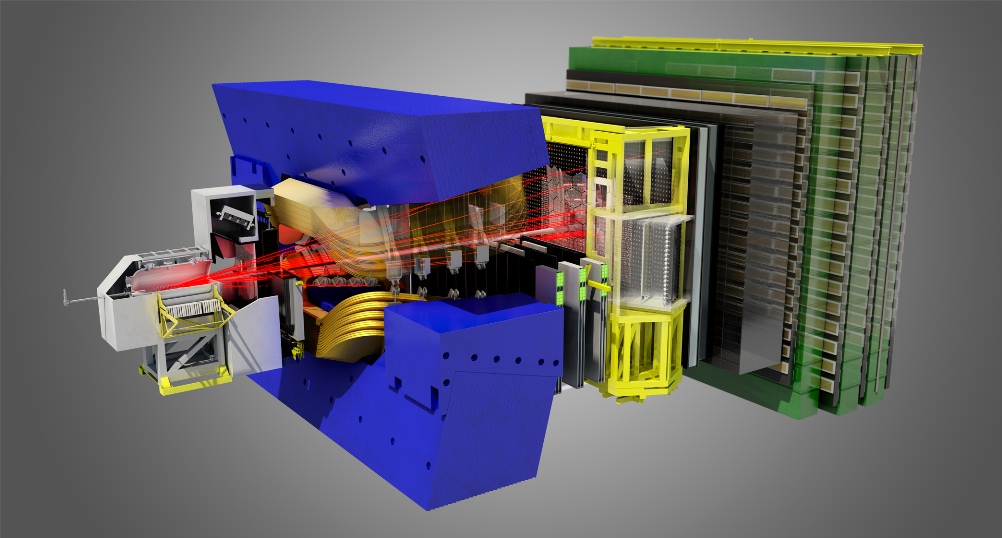
\includegraphics[width=0.77\columnwidth]{chapter3/figs/LHCbDetectorpnglight1}
\caption{The \lhcb detector shown in from a three dimensional perspective.~\label{fig:lhcb:3d} }
\end{figure}
\begin{figure}[p]
\centering
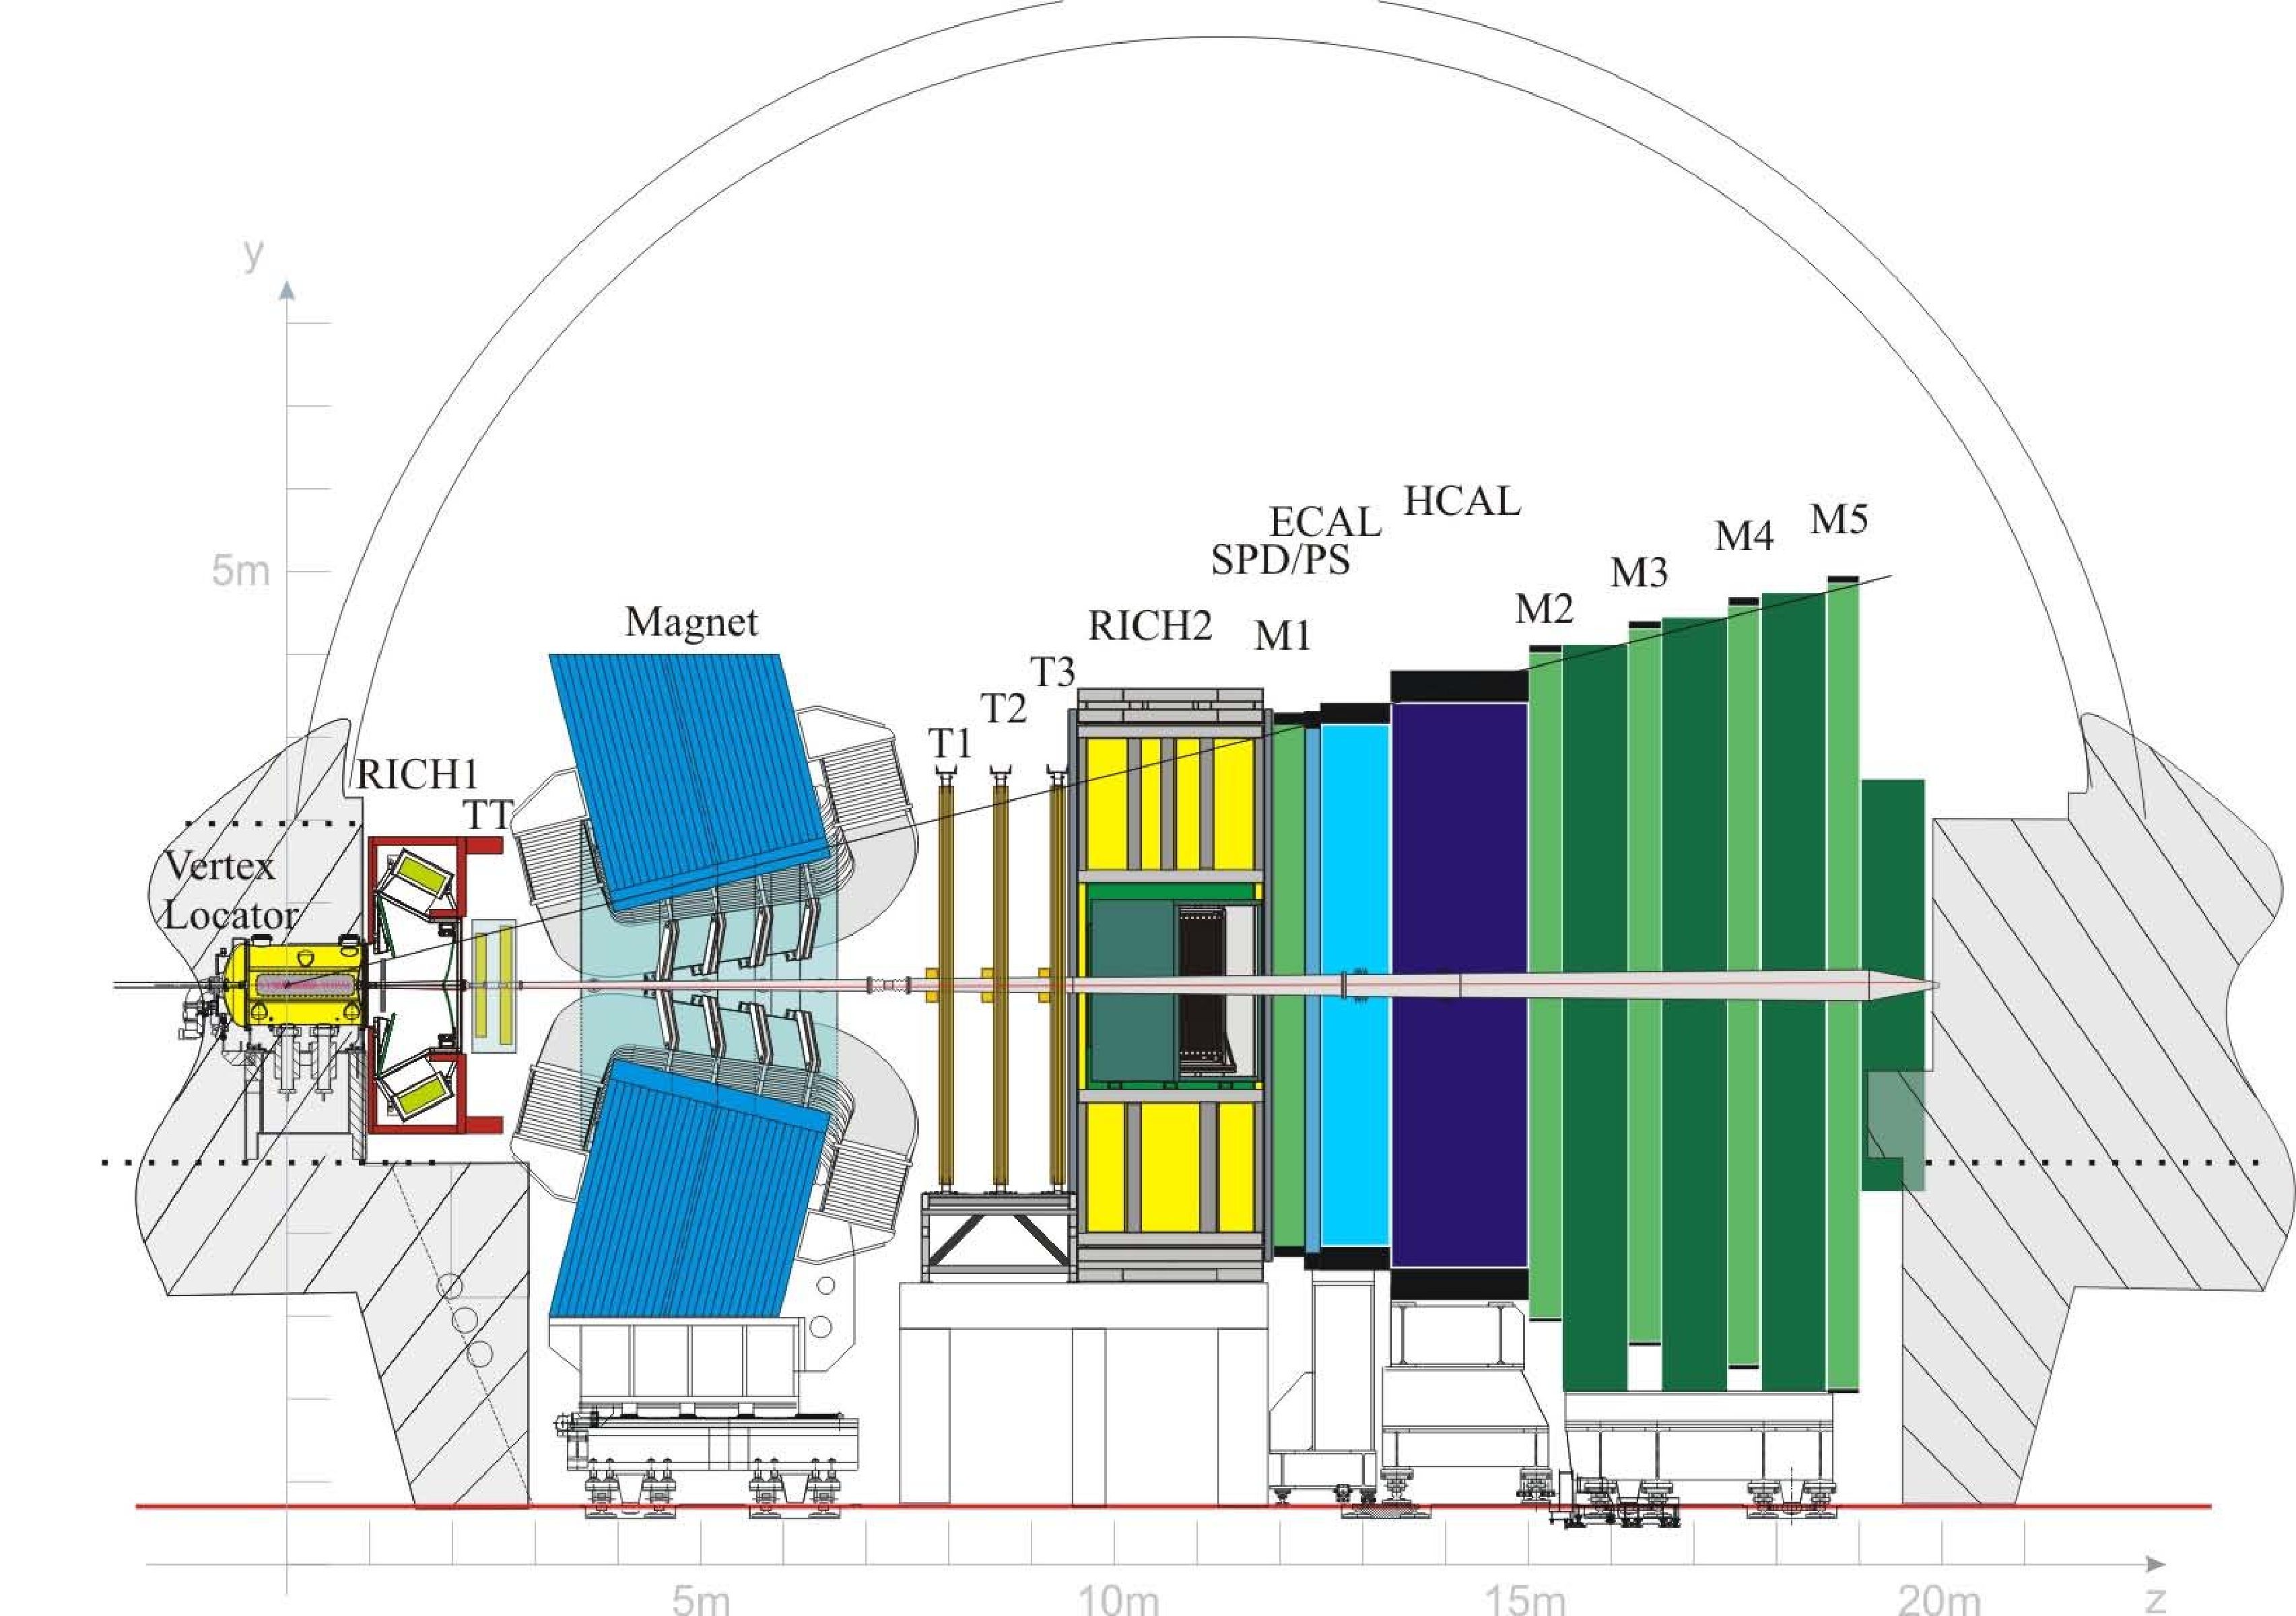
\includegraphics[width=0.77\columnwidth]{chapter3/figs/gene-2008-002_01-1.pdf}
\caption{The \lhcb detector shown side-on. 
The \velo and the interaction point is to the left followed by the first \rich detector. 
The magnet is surrounded by the tracking stations with the second \rich detector to the right of the magnet.
The calorimeters and the muon stations are towards the rear of the detector~\cite{Alves:2008zz}.~\label{fig:lhcb:lhcb} }
\end{figure}

The \lhcb detector consists of a tracking system, detectors for identification of charged hadrons 
and muons and calorimeters to provide energy measurements of charged and neutral particles.
The high precision tracking system
consists of a silicon-strip vertex detector surrounding the $pp$
interaction region, a large-area silicon-strip detector located
upstream of a dipole magnet with a bending power of about
$4{\rm\,Tm}$, and three stations of silicon-strip detectors and straw
drift tubes placed downstream of the magnet. The combined tracking system has a
momentum resolution ($\Delta p/p$) that varies from 0.4\% at 5\gevc to
0.6\% at 100\gevc, and an impact parameter resolution of 20\mum for
tracks with high transverse momentum. Charged hadrons are identified
using two ring-imaging Cherenkov detectors~\cite{arXiv:1211-6759}. 
Photon, electron and hadron candidates are identified by a 
calorimeter system consisting of
scintillating-pad and pre-shower detectors, an electromagnetic
calorimeter and a hadronic calorimeter. Muons are identified by a
system composed of alternating layers of iron and multi-wire
proportional chambers. The trigger consists of a
hardware stage, based on information from the calorimeter and muon
systems, followed by a software stage which applies a full event
reconstruction~\cite{Aaij:2012me}.












